\section{Sincronización de Instrumentos}

En los dos circuitos anteriores se obtuvo la respuesta en frecuencia de los mismos tomando los valores de la amplitud y la fase de la señal de salida a diferentes frecuencias. Luego se graficaron dichos valores en escala semilogarítmica para conseguir una representación gráfica de la función transferencia en módulo y fase. No obstante lo anterior, tener una manera mediante la cual pueda observarse la respuesta en frecuencia de un circuito solamente con un osciloscopio y un generador, puede ser de gran utilidad. Lo anteriormente descrito se realizó de dos maneras diferentes: en primer lugar se usaron dos generadores, el primero para crear una rampa y el segundo para generar el barrido horizontal de la señal. Se configuró el generador para que barriera un gran rango de frecuencias y con el modo XY del osciloscopio se logró visualizar la siguiente imagen: 

\begin{figure}[H]
	\begin{center}
		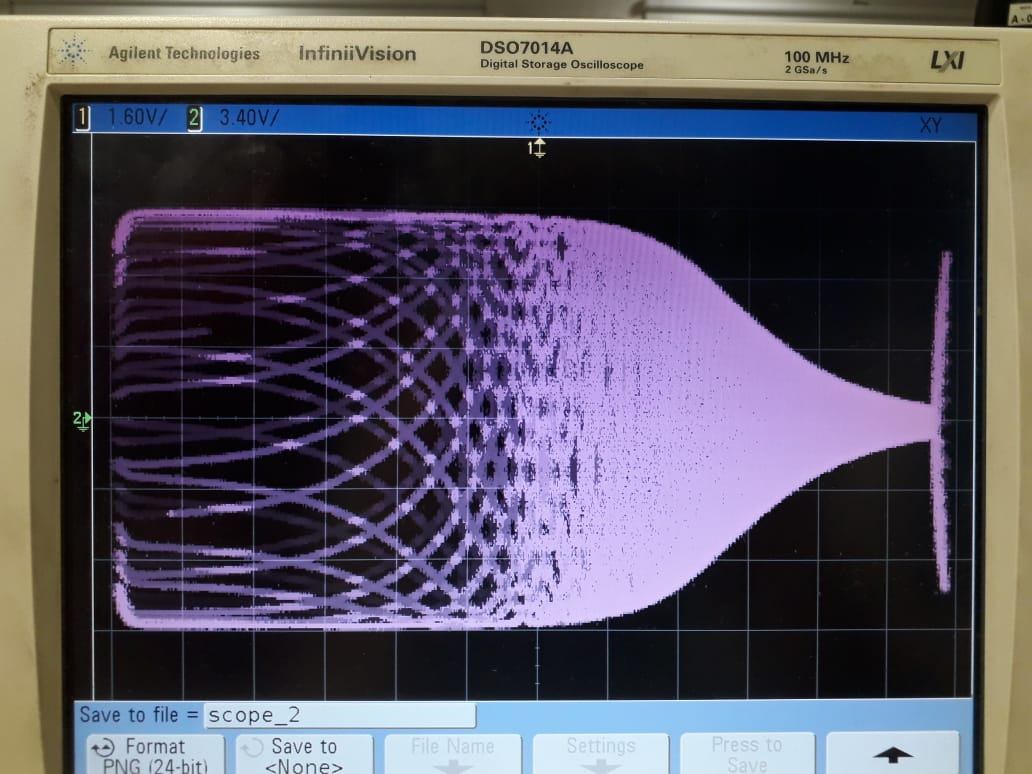
\includegraphics[scale=0.3]{../Mediciones/Fotos/bodeXY.jpg}
	\end{center}
	\caption{Respuesta en frecuencia medida en modo XY}
	\label{fig:bodeXY}
\end{figure}

En segundo lugar se utilizó solamente un generador de funciones y el osciloscopio en modo normal:

\begin{figure}[H]
	\begin{center}
		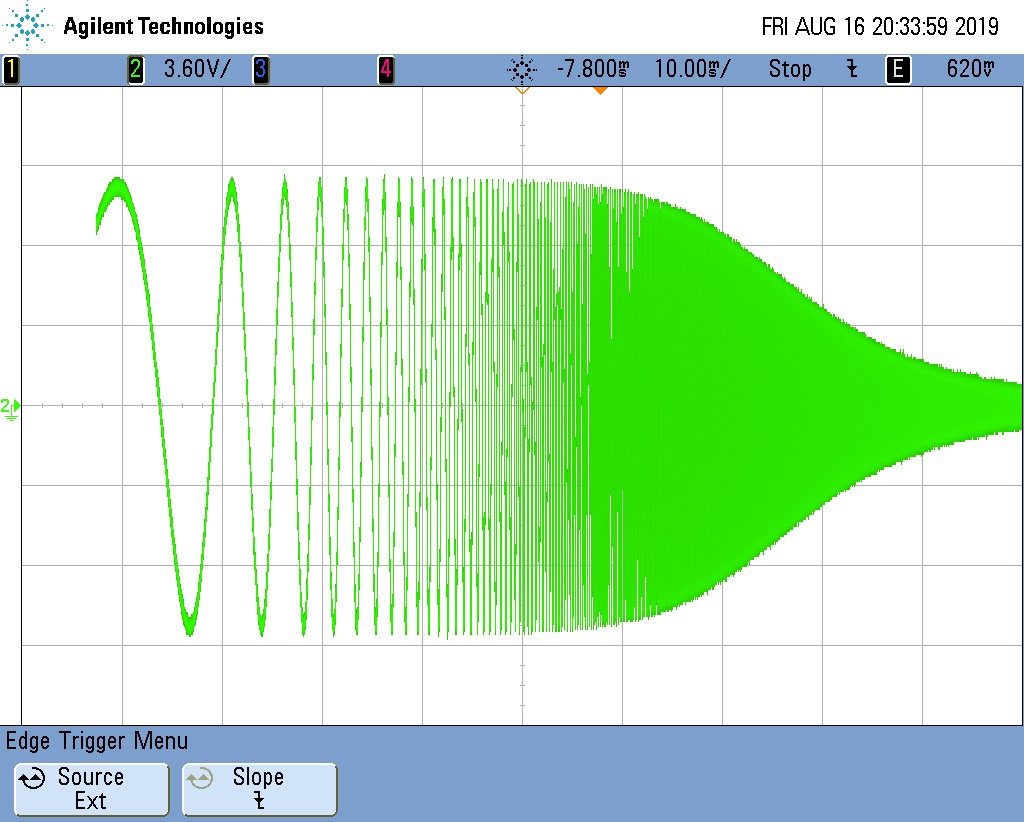
\includegraphics[scale=0.3]{../Mediciones/Fotos/bode_normal.jpg}
	\end{center}
	\caption{Respuesta en frecuencia medida en modo normal}
	\label{fig:bode_normal}
\end{figure}

Es importante aclarar que las imágenes anteriores no son representaciones verdaderas de la respuesta en frecuencia de la señal. Para lograr graficar la salida de un circuito en el dominio de la frecuencia se debería utilizar la Transformada de Fourier, cosa que no puede hacerse con un osciloscopio análogico, pero si en instrumentos digitales que posean dicha función.